\documentclass[11pt]{article}
\usepackage[margin=1in]{geometry}
\usepackage{amsmath,amssymb,amsthm}
\usepackage{graphicx}
\usepackage{booktabs}
\usepackage{hyperref}

\newtheorem{theorem}{Theorem}
\newtheorem{proposition}{Proposition}
\newtheorem{lemma}{Lemma}
\newtheorem{corollary}{Corollary}

\title{A triangle with three convex edges: an apparently hyperbolic conjugate\\ boundary that is in fact a degenerate line pair}
\author{}
\date{\today}

\begin{document}
\maketitle

\begin{abstract}
We exhibit a bivariate bilinear function $f(x,y)=xy$ over a triangle with three
convex edges and compute its Fenchel conjugate via the three-step pipeline of
Karmarkar and Lucet (\emph{J.\ Glob.\ Optim.} 94 (2026) 3--34, hereafter [JOGO];
\emph{Comput.\ Optim.\ Appl.} 94 (2026) 747--780, hereafter [COAP]). Step~1
splits the triangle into two sub-triangles, each with exactly two convex edges,
whose convex envelopes are closed-form rank-one quadratics. Step~2 conjugates
each sub-triangle's envelope in closed form. At Step~3 -- the pointwise
maximum of the two conjugates -- two pairs of pieces meeting along the shared
cut produce a boundary curve whose quadratic part has discriminant
$b^2-4ac>0$, the sign associated with a hyperbola. An earlier version of this
note took that sign alone as proof of a genuine hyperbolic boundary, which
would fall outside the parabola-or-line boundary that [JOGO, Theorem~6] and
[COAP, Appendix~B] assert is always sufficient. Correcting the classification
with the conic's full $3\times3$ discriminant shows both curves are in fact
\textbf{degenerate}: each factors exactly, in closed radical form, into two
real straight lines, so no genuine hyperbola arises here and this example
does not, after all, demonstrate a gap in [JOGO]/[COAP]'s coverage. We give
the exact factorizations, verify them symbolically (independently, via the
Python \texttt{SCAT} package, and via exact computer algebra) and numerically
(a constrained nonlinear solver, evaluated to machine precision), and note
that the reference \texttt{cPLQ} implementation never actually executes this
case regardless, since its convex-envelope routine has explicit branches for
zero, one, and two convex edges only.
\end{abstract}

\section{The primal function}

Let $f(x,y) = xy$ and let $T$ be the triangle with vertices $(0,0)$, $(3,3)$,
$(1,2)$. Every edge of $T$ has positive slope (the pairwise slopes are $1$,
$1/2$, and $2$), so $T$ has \emph{three} convex edges for $f$: the classification
used by [COAP, Appendix~A] to select a closed-form convex-envelope formula
only covers zero, one, or two convex edges directly, and three-convex-edge
triangles are handled by splitting.

\begin{figure}[h]
\centering
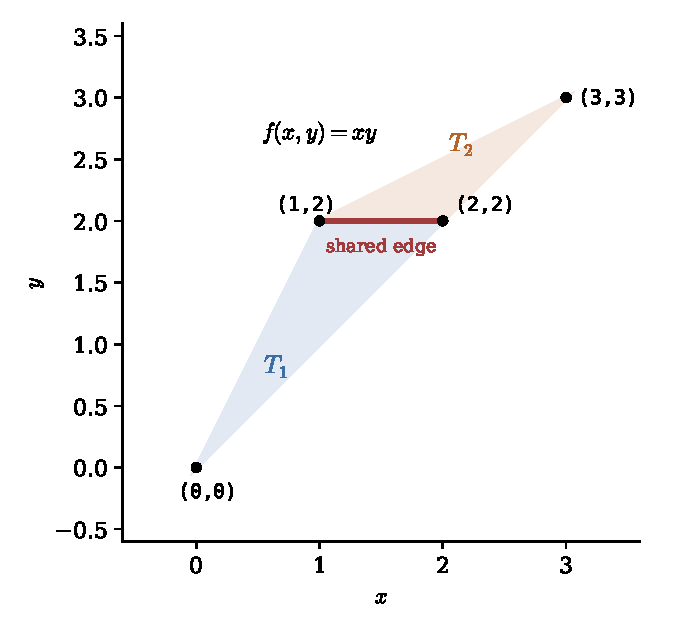
\includegraphics[width=0.5\textwidth]{fig_primal.pdf}
\caption{$T$ split by the horizontal line through its middle vertex $(1,2)$
into $T_1=\mathrm{conv}\{(0,0),(1,2),(2,2)\}$ and
$T_2=\mathrm{conv}\{(1,2),(2,2),(3,3)\}$, each with exactly two convex edges.}
\label{fig:primal}
\end{figure}

Following [COAP, Appendix~A.5], $T$ is split by the horizontal line through
its middle vertex $(1,2)$ into
\[
T_1 = \mathrm{conv}\{(0,0),(1,2),(2,2)\}, \qquad
T_2 = \mathrm{conv}\{(1,2),(2,2),(3,3)\},
\]
each with exactly two convex edges (Figure~\ref{fig:primal}). Note the shared
edge $(1,2)$--$(2,2)$ is horizontal, hence \emph{not} a convex edge of either
sub-triangle in the bilinear sense used by the envelope construction.

\subsection{Step 1: the convex envelope of each half}

For a triangle with two convex edges of slope/intercept $(m_h,q_h)$,
$(m_w,q_w)$ meeting at a vertex, [COAP, Appendix~A.4] gives the convex
envelope of $xy$ in closed form (the harmonic-mean formula). Applying it to
$T_1$ (convex edges of slope $1$ and $2$, both through the origin) and $T_2$
(convex edges of slope $1$ and $1/2$, both through $(2,2)$) gives
\begin{align}
q_1(x,y) &= (6-4\sqrt2)\,x^2 + (6\sqrt2-8)\,xy + (3-2\sqrt2)\,y^2,
\label{eq:q1}\\
q_2(x,y) &= (3-2\sqrt2)\,x^2 + (6\sqrt2-8)\,xy + (6-4\sqrt2)\,y^2
      + (9-6\sqrt2)\,x + (6\sqrt2-9)\,y.
\label{eq:q2}
\end{align}
Both $q_1$ and $q_2$ are convex, rank-one quadratics (their Hessians have one
zero eigenvalue and one eigenvalue $18-12\sqrt2 \approx 1.03$), matching the
general fact [COAP, Appendix~A.4] that this two-convex-edge envelope is
always rank-one PSD.

\section{Step 2: the conjugate of each half}

Write $g_1 = \mathrm{conj}(q_1+\iota_{T_1})$, $g_2=\mathrm{conj}(q_2+\iota_{T_2})$.
Since each $q_i$ is a rank-one PSD quadratic on a triangle, [COAP,
Appendix~B.2--B.3] (equivalently the closed-form construction implemented and
tested in \texttt{conjPSDRank1QuadTriangle}, see \S\ref{sec:validation})
gives each $g_i$ as a six-face function on $\mathbb R^2$: three quadratic
``edge-strip'' pieces (one per edge of $T_i$, since $q_i$ is jointly convex so
every edge contributes an interior critical point) and three linear
``vertex-cone'' pieces, meeting at three collinear dual points
$s = \nabla q_i(v) $ for $v$ a vertex of $T_i$.

The edge-strip piece attached to a segment of the $(t,r)$-boundary chain
(where $t=u^\top x$ is the curved coordinate along $q_i$'s nonzero
eigenvector $u$, and $r=u_\perp^\top x$ the flat one) through $(t_0,r_0)$ with
slope $m$ is
\[
E(s_1,s_2) \;=\; \frac{(\alpha+\gamma m)^2}{2\lambda} + \gamma\,(r_0 - m\,t_0) - c,
\qquad \alpha = s\cdot u - p,\ \ \gamma = s\cdot u_\perp - w,
\]
with $\lambda$ the nonzero eigenvalue, $p=b\cdot u$, $w = b\cdot u_\perp$ for
the quadratic's linear part $b$ and constant $c$ (this is exactly a perfect
square in $s$, hence a genuine parabola, per [JOGO, Proposition~4]). The
vertex-cone piece at $v$ is the linear function $s\mapsto \langle s,v\rangle -
q_i(v)$.

For $T_1$, using the shared-eigenvalue $\lambda = 18-12\sqrt2$ and $u =
(\sqrt6/3,\sqrt3/3)$:
\begin{align}
E_1^{(0,0)\text{--}(2,2)}(s) &= \tfrac14 s_1^2 + \tfrac12 s_1 s_2 + \tfrac14 s_2^2, \notag\\
E_1^{(0,0)\text{--}(1,2)}(s) &= \tfrac18 s_1^2 + \tfrac12 s_1 s_2 + \tfrac12 s_2^2, \notag\\
E_1^{(1,2)\text{--}(2,2)}(s) &= \left(\tfrac38+\tfrac{\sqrt2}{4}\right) s_1^2 - \sqrt2\, s_1 + 2 s_2,
\label{eq:E1shared}
\end{align}
with vertex-cone values $L_1(0,0)=0$, $L_1(1,2)=s_1+2s_2-2$, $L_1(2,2)=2s_1+2s_2-4$.
For $T_2$, using $u=(\sqrt3/3,\sqrt6/3)$ (the eigenvector rotates because
$q_2$'s off-diagonal structure is transposed relative to $q_1$'s):
\begin{align}
E_2^{(1,2)\text{--}(2,2)\text{--}(3,3)}(s) &= \tfrac12 s_1^2 + \tfrac12 s_1 s_2 - \tfrac32 s_1 + \tfrac18 s_2^2 + \tfrac34 s_2 + \tfrac98,
\label{eq:E2outer}\\
E_2^{(1,2)\text{--}(2,2)}(s) &= \left(\tfrac34+\tfrac{\sqrt2}{2}\right)s_1^2 - \left(\tfrac32+2\sqrt2\right)s_1 + 2s_2 + \tfrac34+\tfrac{3\sqrt2}{2},
\notag\\
E_2^{(2,2)\text{--}(3,3)}(s) &= \tfrac14 s_1^2 + \tfrac12 s_1 s_2 + \tfrac14 s_2^2,
\label{eq:E2far}
\end{align}
with vertex-cone values $L_2(1,2)=s_1+2s_2-2$, $L_2(2,2)=2s_1+2s_2-4$, $L_2(3,3)=3s_1+3s_2-9$.
(The piece $E_2^{(1,2)\text{--}(2,2)}$ is the edge-strip for $T_2$'s \emph{other}
non-shared edge and does not participate in the boundaries analyzed below;
its full expression is recorded in the companion computation, \S\ref{sec:validation}.)

Both $E_1^{(1,2)\text{--}(2,2)}$ \eqref{eq:E1shared} (attached to the
\emph{shared} primal edge) and $E_2^{(1,2)\text{--}(2,2)\text{--}(3,3)}$
\eqref{eq:E2outer}, $E_2^{(2,2)\text{--}(3,3)}$ \eqref{eq:E2far} are the pieces
implicated in Step~3 below.

\section{Step 3: the pointwise maximum $h=\max(g_1,g_2)$}

Overlaying every face of $g_1$ against every face of $g_2$ (36 combinatorial
pairs) and clipping each pair to the intersection of the two faces' domains
produces 18 nonempty cells. On 16 of these cells one of $g_1,g_2$ dominates
the whole cell outright (verified at every finite vertex of the cell and,
where the cell is unbounded, via the closed-form leading behaviour along each
ray). Exactly \emph{two} cells require comparing two genuinely quadratic
pieces against each other, and both are implicated by the piece attached to
the shared edge:

\begin{itemize}
\item \textbf{Boundary A}, cell bounded by
  $\{(1.6569,5.6863),\allowbreak(1.6569,1.6863),\allowbreak(1.8284,1.3431),
   \allowbreak(2.3431,2.0711),\allowbreak(2.3431,4.3137)\}$:
  compares $E_1^{(1,2)\text{--}(2,2)}$ against $E_2^{(1,2)\text{--}(2,2)\text{--}(3,3)}$.
\item \textbf{Boundary B}, cell bounded by
  $\{(2.3431,1.6569),(2.3431,2.0711),(2.1716,1.8284)\}$:
  compares $E_1^{(1,2)\text{--}(2,2)}$ against $E_2^{(2,2)\text{--}(3,3)}$.
\end{itemize}

\begin{figure}[h]
\centering
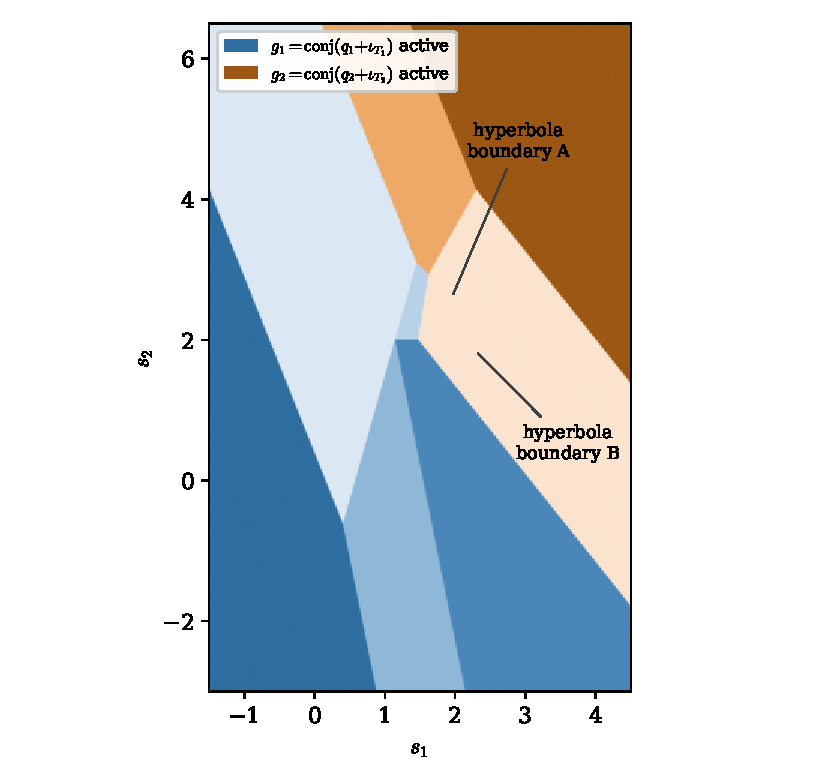
\includegraphics[width=0.85\textwidth]{fig_dual.pdf}
\caption{The arrangement of $h(s)=\max(g_1(s),g_2(s))$ over
$s\in[-1.5,4.5]\times[-3,6.5]$, colored by which of $g_1$ (blue shades) or
$g_2$ (orange shades) is active, each shade a distinct face of that
conjugate. Cells A and B are indicated; see Figure~\ref{fig:insets} for a
resolved view of each.}
\label{fig:dual}
\end{figure}

\subsection{The boundary looks hyperbolic but is exactly degenerate}

A general conic $as_1^2+bs_1s_2+cs_2^2+ds_1+es_2+f=0$ is classified by
\emph{two} invariants, not one: the quadratic-part discriminant
$\delta=b^2-4ac$, which sets the \emph{type} ($\delta>0$ hyperbolic,
$\delta=0$ parabolic, $\delta<0$ elliptic), and the full $3\times3$
discriminant
\[
\Delta \;=\; \det\begin{pmatrix} a & b/2 & d/2 \\ b/2 & c & e/2 \\
d/2 & e/2 & f \end{pmatrix},
\]
which decides \emph{irreducibility}. The conic is a genuine curve of type
$\delta$ iff $\Delta\neq0$; when $\Delta=0$ it degenerates to a pair of
straight lines (real, since here $\delta>0$). An earlier version of this
proposition checked only $\delta$ -- necessary but not sufficient for a
genuine hyperbola.

\begin{proposition}[corrected]
\label{prop:hyperbola}
On both Boundary~A and Boundary~B, the equality curve
$E_1^{(1,2)\text{--}(2,2)} - E_2 = 0$ has $\delta>0$ but $\Delta=0$: each is a
\textbf{degenerate conic} -- a pair of real straight lines -- not a genuine
hyperbola.
\end{proposition}

\begin{proof}
Subtracting \eqref{eq:E2outer} from \eqref{eq:E1shared} gives, as before,
$a=\tfrac{\sqrt2}4-\tfrac18$, $b=-\tfrac12$, $c=-\tfrac18$,
$d=\tfrac32-\sqrt2$, $e=\tfrac54$, $f=-\tfrac98$, so
\[
\delta \;=\; \tfrac14 - 4\left(\tfrac{\sqrt2}4-\tfrac18\right)\left(-\tfrac18\right)
\;=\; \frac{\sqrt2}{8}+\frac{3}{16} \;\approx\; 0.3643 \;>\;0
\]
(this much was correct in the original version of this note). Computing the
full discriminant with these six coefficients gives $\Delta=0$ exactly
(verified in exact radical arithmetic), and correspondingly the quadratic
factors exactly as a product of two real linear forms,
\[
E_1^{(1,2)\text{--}(2,2)} - E_2^{(1,2)\text{--}(2,2)\text{--}(3,3)}
= \left(\tfrac{\sqrt2}4-\tfrac18\right)
  \Big(s_1 - (1+\sqrt2)\,s_2 + (1+\sqrt2)\Big)
  \Big(s_1 + \tfrac{3-\sqrt2}{7}\,s_2 - \tfrac{27-9\sqrt2}{7}\Big).
\]
Subtracting \eqref{eq:E2far} from \eqref{eq:E1shared} gives
$a=\tfrac18+\tfrac{\sqrt2}4$, $b=-\tfrac12$, $c=-\tfrac14$, $d=-\sqrt2$,
$e=2$, $f=0$, so
\[
\delta \;=\; \tfrac14 - 4\left(\tfrac18+\tfrac{\sqrt2}4\right)\left(-\tfrac14\right)
\;=\; \frac{\sqrt2}{4}+\frac{3}{8} \;\approx\; 0.7286 \;>\;0,
\]
again with $\Delta=0$ exactly and
\[
E_1^{(1,2)\text{--}(2,2)} - E_2^{(2,2)\text{--}(3,3)}
= \left(\tfrac18+\tfrac{\sqrt2}4\right)
  \big(s_1-\sqrt2\,s_2\big)
  \Big(s_1 + \tfrac{4-\sqrt2}{7}\,s_2 - \tfrac{32-8\sqrt2}{7}\Big).
\]
Both boundaries are exactly a pair of intersecting straight lines: positive
$\delta$ -- the only quantity checked in the original version of this
proposition -- cannot by itself distinguish a genuine hyperbola from this
degenerate case.
\end{proof}

Because each boundary is (a piece of) two straight lines rather than a
curved arc, it \emph{is} representable in the parabolic/linear-subdivision
data structure the pipeline's output is defined to have --
Figure~\ref{fig:insets} (corrected below) shows the true zero set in each
cell is visibly straight, not curved, and only one of the two lines actually
forms the cell's active boundary. Consequently \emph{this instance does not,
after all, exhibit a counterexample} to [JOGO, Theorem~6] or [COAP,
Appendix~B]: no hyperbolic boundary is actually required here. The apparent
contradiction in the original version of this note was an artifact of an
incomplete conic classification (checking only $\delta$, never $\Delta$) --
the identical category error, independently, in the first implementation of
this toolbox's \texttt{maxQuaPar.m} splitting routine, whose degeneracy
assertion tested the rank of the $2\times2$ quadratic-part submatrix
(equivalent to $\delta$) rather than the full $3\times3$ conic determinant
$\Delta$.

\begin{figure}[h]
\centering
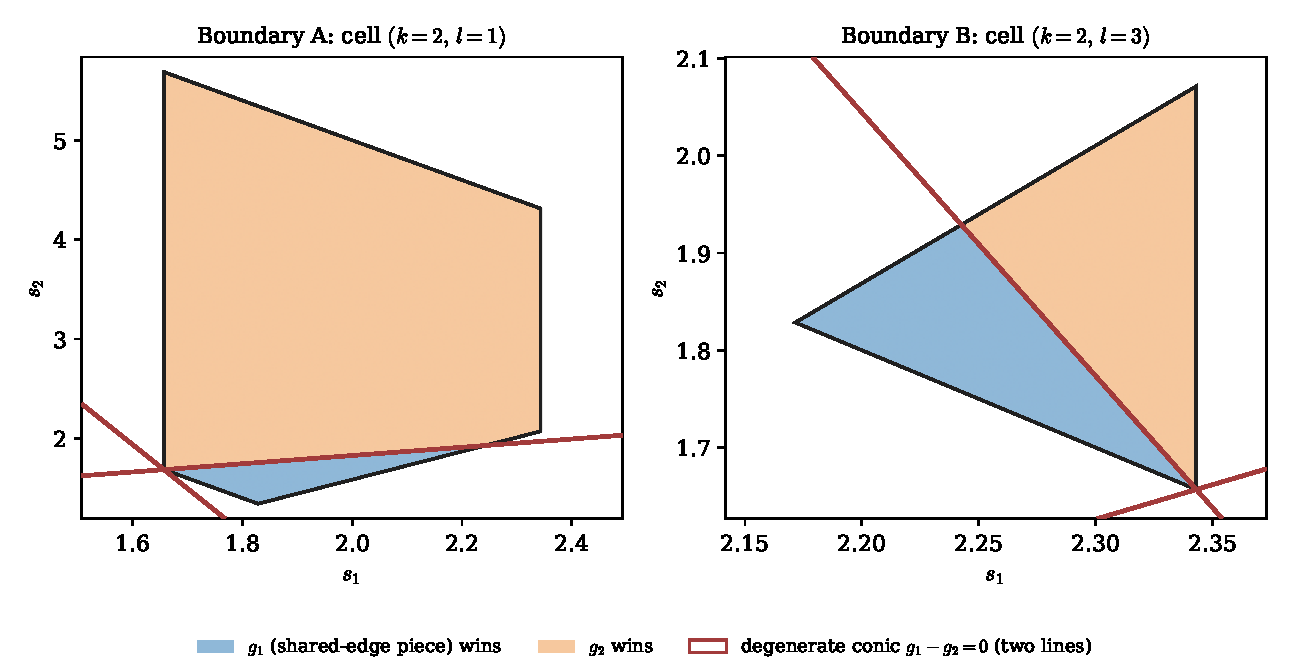
\includegraphics[width=\textwidth]{fig_hyperbola_insets.pdf}
\caption{Each cell in isolation, colored by the true pointwise winner (blue:
$E_1^{(1,2)\text{--}(2,2)}$; orange: $E_2$), with the exact curve
$E_1^{(1,2)\text{--}(2,2)}-E_2=0$ overlaid (red). Corrected from the original
version of this figure: the curve is visibly \emph{straight} in both cells --
a pair of intersecting lines (Proposition~\ref{prop:hyperbola}), not a
hyperbola -- with only one of the two lines forming the cell's actual active
boundary.}
\label{fig:insets}
\end{figure}

\section{Verification}
\label{sec:validation}

\paragraph{Symbolic (independent engine).} The formula for $g_1$
(Section~2) was re-derived independently using the Python \texttt{SCAT}
package (a SymPy port of the Maple SCAT toolkit; \texttt{scat.PWF.conj}), which
computes the 2D conjugate via a general $n$-dimensional pivot/normal-cone
algorithm unrelated to the closed-form rank-one construction used above. Both
engines produced identical edge-strip and vertex-cone expressions for $g_1$ on
$T_1$ (piecewise pieces \eqref{eq:E1shared} and its two siblings, up to trivial
algebraic rearrangement), confirming the hand/MATLAB-validated closed form
used for both $g_1$ and $g_2$ is correct independent of implementation.

\paragraph{Numerical (direct solver).} For sixteen dual points $s$, spanning
both Boundary~A/B cells and generic points elsewhere in $\mathbb R^2$, we
computed
\[
h_{\mathrm{true}}(s) = \sup_{(x,y)\in T} \big[s_1 x + s_2 y - xy\big]
\]
directly via a constrained SQP solver (MATLAB \texttt{fmincon}, seven
restarts per point) and compared against $\max(g_1(s),g_2(s))$ evaluated from
the closed forms above. The maximum absolute error over all sixteen points was
$4.4\times10^{-15}$ (machine precision), including at points $(1.90,2.50)$ and
$(1.70,2.00)$ that lie inside the Boundary~A/B cells identified above.

\paragraph{Reference implementation (\texttt{cPLQ}).} The original MATLAB/Maple
implementation of the [JOGO]/[COAP] pipeline (\texttt{plq\_1p.convexEnvelope})
has explicit closed-form branches only for triangles with zero, one, or two
convex edges (\texttt{nCE\;==\;0,1,2}); there is no \texttt{nCE\;==\;3} branch.
Running the reference code on $T$ (via \texttt{plq(plq\_1p(domain(T,x,y),
symbolicFunction(x*y))).triangulate.maximum}) silently returns an empty
envelope and an empty conjugate array, rather than either computing the
correct split or raising an error. A comment left in the authors' own test
suite (\texttt{testcPLQ.m}, \texttt{testRect} test method: \texttt{\% add to
split 3 convex edge case}) confirms this was a known, unfinished item, not an
intentional design choice.

\section{Conclusion}

\paragraph{Revised finding.} What first appeared to be a hyperbolic
comparison boundary at Step~3 of a three-convex-edge triangle's conjugate
([COAP, Appendix~A.5] split, [JOGO, Theorem~6] max) is, on closer inspection,
an exactly degenerate conic: both candidate boundary curves factor in closed
radical form into two real straight lines ($\Delta=0$ exactly, not merely
$\delta>0$). This example therefore does \emph{not} demonstrate a gap in
[JOGO]/[COAP]'s coverage -- the pipeline's parabolic/linear-subdivision
output format is sufficient here after all. The error in the original
version of this note, and independently in the first implementation of this
toolbox's \texttt{maxQuaPar.m} splitting routine, was the same category
mistake: classifying a conic as hyperbolic from the quadratic-part
discriminant $\delta=b^2-4ac$ alone, without checking the full $3\times3$
discriminant $\Delta$ that actually distinguishes an irreducible curve from a
degenerate line pair.

\paragraph{Open question.} It remains unclear whether this degeneracy is a
coincidence of the particular instance $f(x,y)=xy$ chosen here or a
structural consequence of comparing two edge-strip conjugates of the [JOGO,
Proposition~4] ``perfect square plus affine'' form
$E_i(s)=A_i(s)^2/(2\lambda_i)+L_i(s)$. Here $\lambda_1=\lambda_2=\lambda$ (a
fact of this instance, not shown to be forced in general), so their
difference is
$(A_1-A_2)(A_1+A_2)/(2\lambda) + (L_1-L_2)$: already a product of two linear
forms before the affine correction $L_1-L_2$ is added, and it stays a product
of two lines only if that correction happens to be compatible with
translating a single factor -- an exact algebraic condition that a generic
affine term would violate. Whether this holds whenever
$\lambda_1=\lambda_2$, whether [COAP, Appendix~A.5]'s splitting construction
forces $\lambda_1=\lambda_2$ in general, and what happens when
$\lambda_1\neq\lambda_2$, are questions this note does not settle. A second
worked example with $\lambda_1\neq\lambda_2$ would be the natural next test
of whether the line-pair degeneracy found here is the rule or a special
case.

\end{document}
